% Define block styles
\tikzstyle{block} = [rectangle, fill=white, text centered, minimum height=0.5em, rounded corners=true]
\tikzstyle{blockBox} = [draw, rectangle, fill=white, minimum height=2.8cm, minimum width=6.0cm, text width=1em, text centered, rounded corners=true]

\tikzstyle{blockSupP} = [draw, rectangle, fill=red1!20,   minimum height=0.52cm, minimum width=1.3cm, text width=1em, text centered, rounded corners=true]
\tikzstyle{blockSupM} = [draw, rectangle, fill=green1!20, minimum height=0.52cm, minimum width=3.1cm, text width=3.1cm, text centered, rounded corners=true]
\tikzstyle{blockSupS} = [draw, rectangle, fill=blue1!20,  minimum height=0.52cm, minimum width=1.3cm, text width=1em, text centered, rounded corners=true]
\tikzstyle{blockSup}  = [draw, rectangle, fill=red1!20,   minimum height=0.52cm, minimum width=3.1cm, text width=3.1cm, text centered, rounded corners=true]

\tikzstyle{blockCon} = [draw, rectangle, fill=white, minimum height=0.5cm, minimum width=1cm, text width=0.6cm, text centered, rounded corners=true]
\tikzstyle{blockP} = [draw, rectangle, fill=red1!40, minimum height=0.52cm, minimum width=0.6cm, text width=1em, text centered, rounded corners=true]
\tikzstyle{blockM} = [draw, rectangle, fill=green1!40, minimum height=0.52cm, minimum width=0.6cm, text width=1em, text centered, rounded corners=true]
\tikzstyle{blockS} = [draw, rectangle, fill=blue1!40, minimum height=0.52cm, minimum width=0.6cm, text width=1em, text centered, rounded corners=true]
\tikzstyle{blockL} = [draw, rectangle, fill=black!20, minimum height=0.52cm, minimum width=0.6cm, text width=1em, text centered, rounded corners=true]
\tikzstyle{arrow} = [draw, -latex]
\tikzstyle{line} = [draw]

\definecolor{red1}{RGB}{160,0,0}
\definecolor{green1}{RGB}{0,160,0}
\definecolor{blue1}{RGB}{0,0,160}

\pgfdeclareimage[width=0.6cm]{hand}{./figures/sec/robothand.jpg}

	      
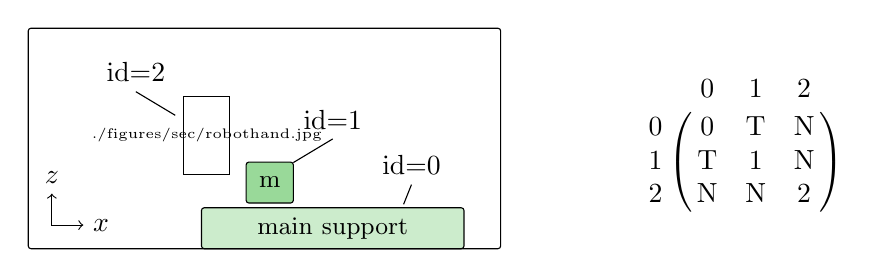
\begin{tikzpicture}[node distance=6em, auto]
	%%%%%%%%%%%%%%%%%%%%%%%%%%%%%%%%%%%%%%%%%%%%%%%%%%%%%%%%%%%%%%%%%%%%%%%%%%%%%%%%%%%%%%%%%%%%%%%%%%%%%%
	% Panel
	\node [blockBox] (p11) {};

	\node[above right, xshift=2.2cm, blockSupM, minimum width=3cm] at (p11.south west) (p11_Sup) {\small{main support}};
	\node[above of=p11_Sup, blockM, node distance=0.58cm, xshift=-0.8cm] (p11_m) {\small{m}};
	\node[left of=p11_m, node distance=0.8cm, yshift=0.6cm] (p11_h) {\pgfuseimage{hand}};

    % Text
    \node[right of=p11_Sup, node distance=0.8cm, xshift=0.2cm, yshift=0.8cm] (p11_Sup_t) {id=0};
    \node[right of=p11_m,   node distance=0.8cm, xshift=0.0cm, yshift=0.8cm] (p11_m_t) {id=1};
    \node[left of=p11_h,    node distance=0.8cm, xshift=-0.1cm, yshift=0.8cm] (p11_h_t) {id=2};

    % Lines
    \draw[line] (p11_Sup_t.south) to ++(-0.1cm,-0.25cm);
    \draw[line] (p11_m_t.south) to ++(-0.5cm,-0.3cm);
    \draw[line] (p11_h_t.south) to ++( 0.5cm,-0.3cm);

    \draw [<->] (-2.7cm,-0.7cm) node (yaxis) [above] {$z$}
                |- (-2.3cm,-1.1cm) node (xaxis) [right] {$x$};


	%%%%%%%%%%%%%%%%%%%%%%%%%%%%%%%%%%%%%%%%%%%%%%%%%%%%%%%%%%%%%%%%%%%%%%%%%%%%%%%%%%%%%%%%%%%%%%%%%%%%%%
	% Matrix

    \node[block, right of=p11_m, yshift=0.5cm, node distance=6.0cm] (p31) {
      $\bordermatrix{
          & 0 & 1 & 2\cr
        0 & 0           & \textup{T}    & \textup{N}\cr
        1 & \textup{T}  & 1             & \textup{N}\cr
        2 & \textup{N}  & \textup{N}    & 2\cr        
      }$
    };
\end{tikzpicture}
